%!TEX program = xelatex
%\documentclass[UTF8,10pt]{ctexbeamer}%,aspectratio=169 %画面比例16:9%
\documentclass[10pt]{beamer}
\usepackage[UTF8]{ctex}

\usetheme[
%sidebar, % 会在每页左侧加上导航栏,参考 The AAU Sidebar Beamer Theme 设置
% xdblue, % 不选会默认西电红色调,选上会将主题设置为西电蓝色调
% english % 选上,会将图表等标题还原回英文标题
%hidetitle,
%hideauthor,
%hideinstitute,
 ]{XDUstyle}

\graphicspath{{figures/}}
%\usetheme{Madrid}
%\useoutertheme[subsection=false]{miniframes}

\AtBeginDocument{%
    \title{基于优化集成学习与空间相关\\滤波的视觉目标跟踪}
    %\subtitle{子标题}
    \author[赵素杰]{%
        \begin{tabular}{ll}
            学\qquad{}生:& 赵素杰 \tabularnewline
            指导老师:& 田小林~副教授
        \end{tabular}
    }
    \institute[智能所]{西安电子科技大学\\“智能感知与图像理解”实验室} % 中括号部分为导航栏底所用尽可能精简
    \date{\today}% 时间可自行设置
}	
\begin{document}%
{%\xdbg
  \frame[plain,noframenumbering]{\titlepage}}%首页标题页

%\part{内容}
\section*{目录}
  \frame {
    \frametitle{\secname}
   % \begin{multicols}{2}
    \tableofcontents[hidesubsections,sections={<1-6>}]
  %\end{multicols}
      }

  \section{研究背景及意义}

\subsection{视觉跟踪}

\begin{frame}{视觉跟踪的研究内容}

\begin{block}{}
    视觉跟踪即连续不断地定位运动目标。给定第一帧中的目标位置,跟踪算法能够在视频中预测出目标运动。
\end{block}
\begin{figure}[htp]
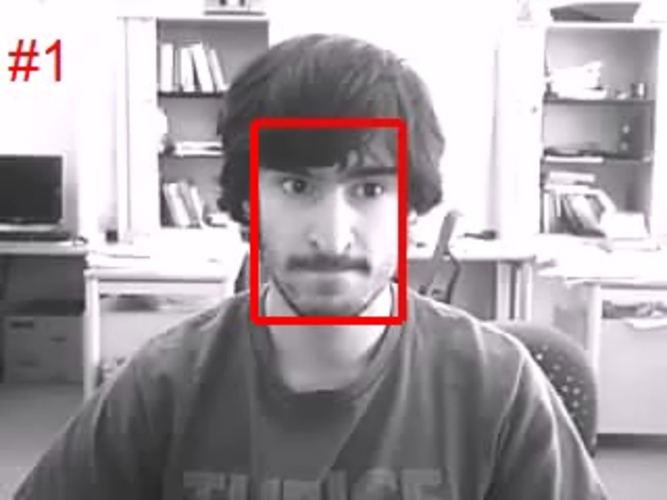
\includegraphics[width=0.25\linewidth,height=0.2\linewidth]{FaceOcc2.pdf}
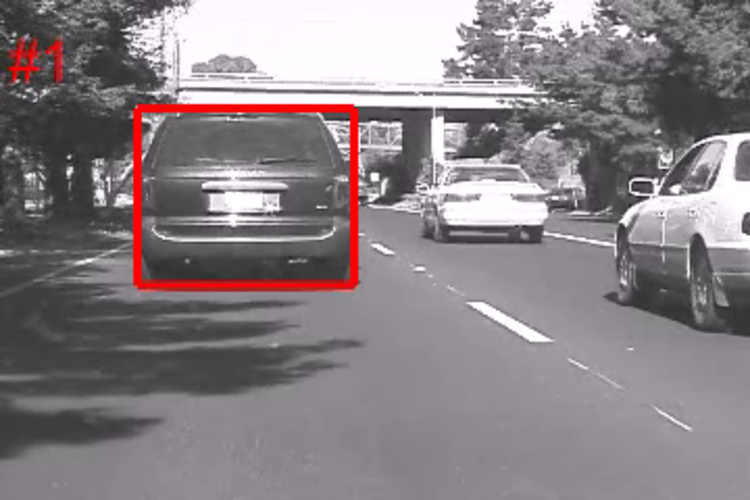
\includegraphics[width =0.25\linewidth,height=0.2\linewidth]{Car4.pdf}
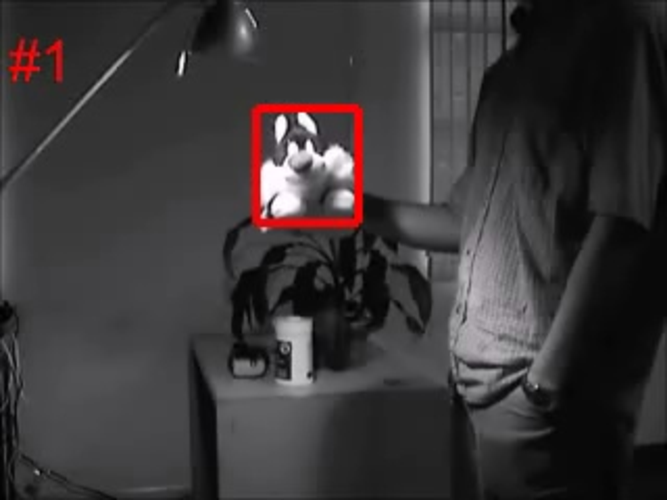
\includegraphics[width =0.25\linewidth,height=0.2\linewidth]{Sylvester.pdf}
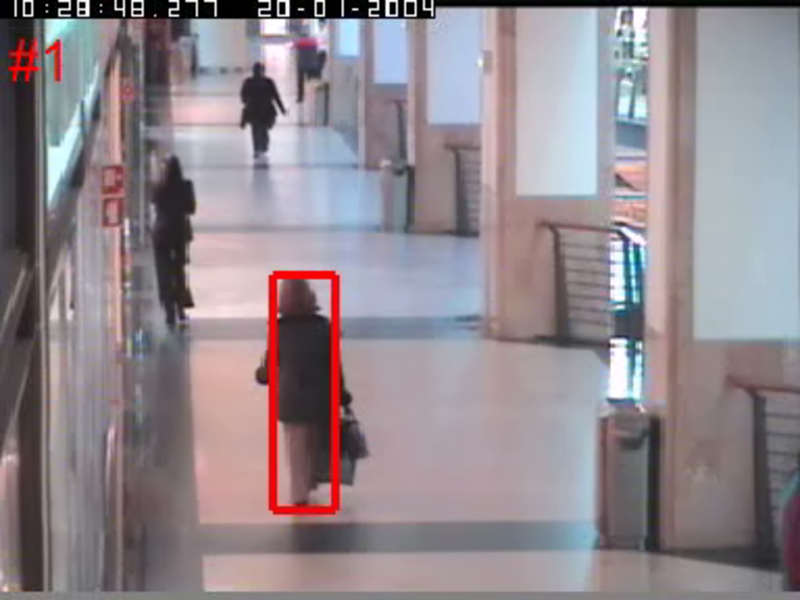
\includegraphics[width =0.25\linewidth,height=0.2\linewidth]{Walking2.pdf}
\caption{单目标视觉跟踪(无模型)}
\end{figure}
\end{frame}


\begin{frame}{视觉跟踪的应用}
    \begin{block}{}
跟踪是视觉监控系统的主要组成部分;在自动驾驶系统中,实时跟踪车辆并预测其运动是非常重要的;自主机器人跟踪它们周围的对象,以便识别人的意图;医学数据分析需要使用可变形模板来跟踪非刚性结构。
\end{block}
\begin{figure}[htp]
%\begin{minipage}{1.06\textwidth}
\subfloat[自动驾驶]{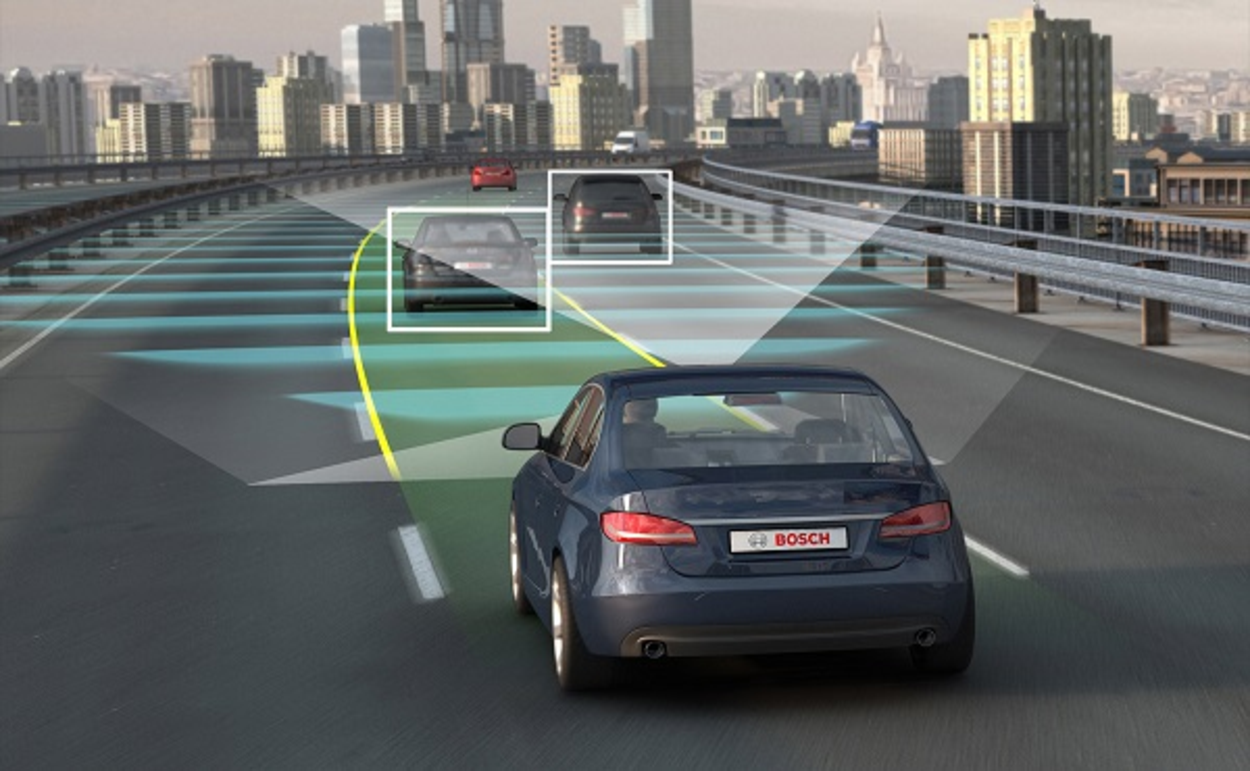
\includegraphics[width=0.25\linewidth,height=0.2\linewidth]{AutonomousCar.pdf}}
\subfloat[人机交互]{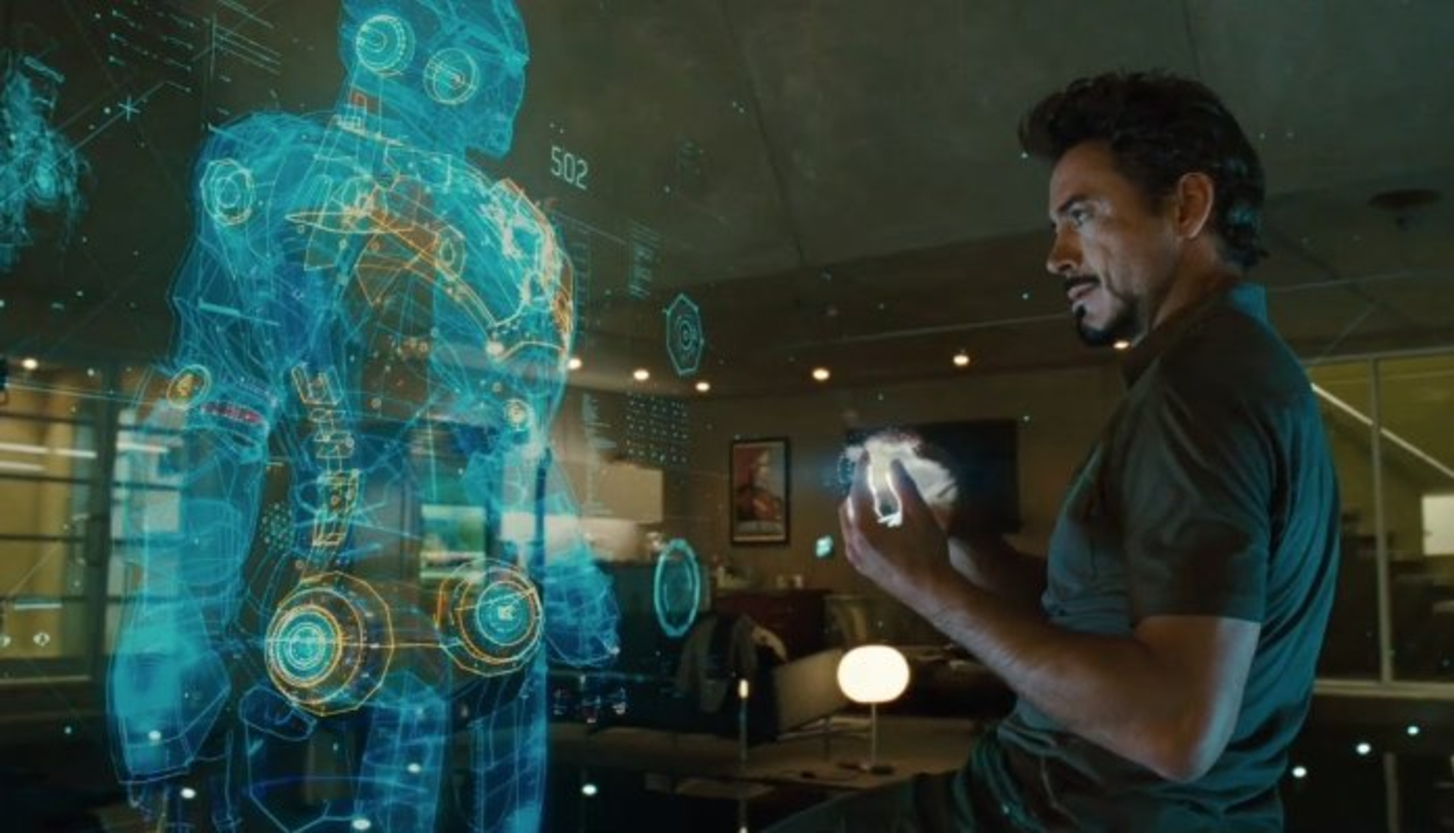
\includegraphics[width =0.25\linewidth,height=0.2\linewidth]{HumanComputerInteraction.pdf}}
\subfloat[运动分析]{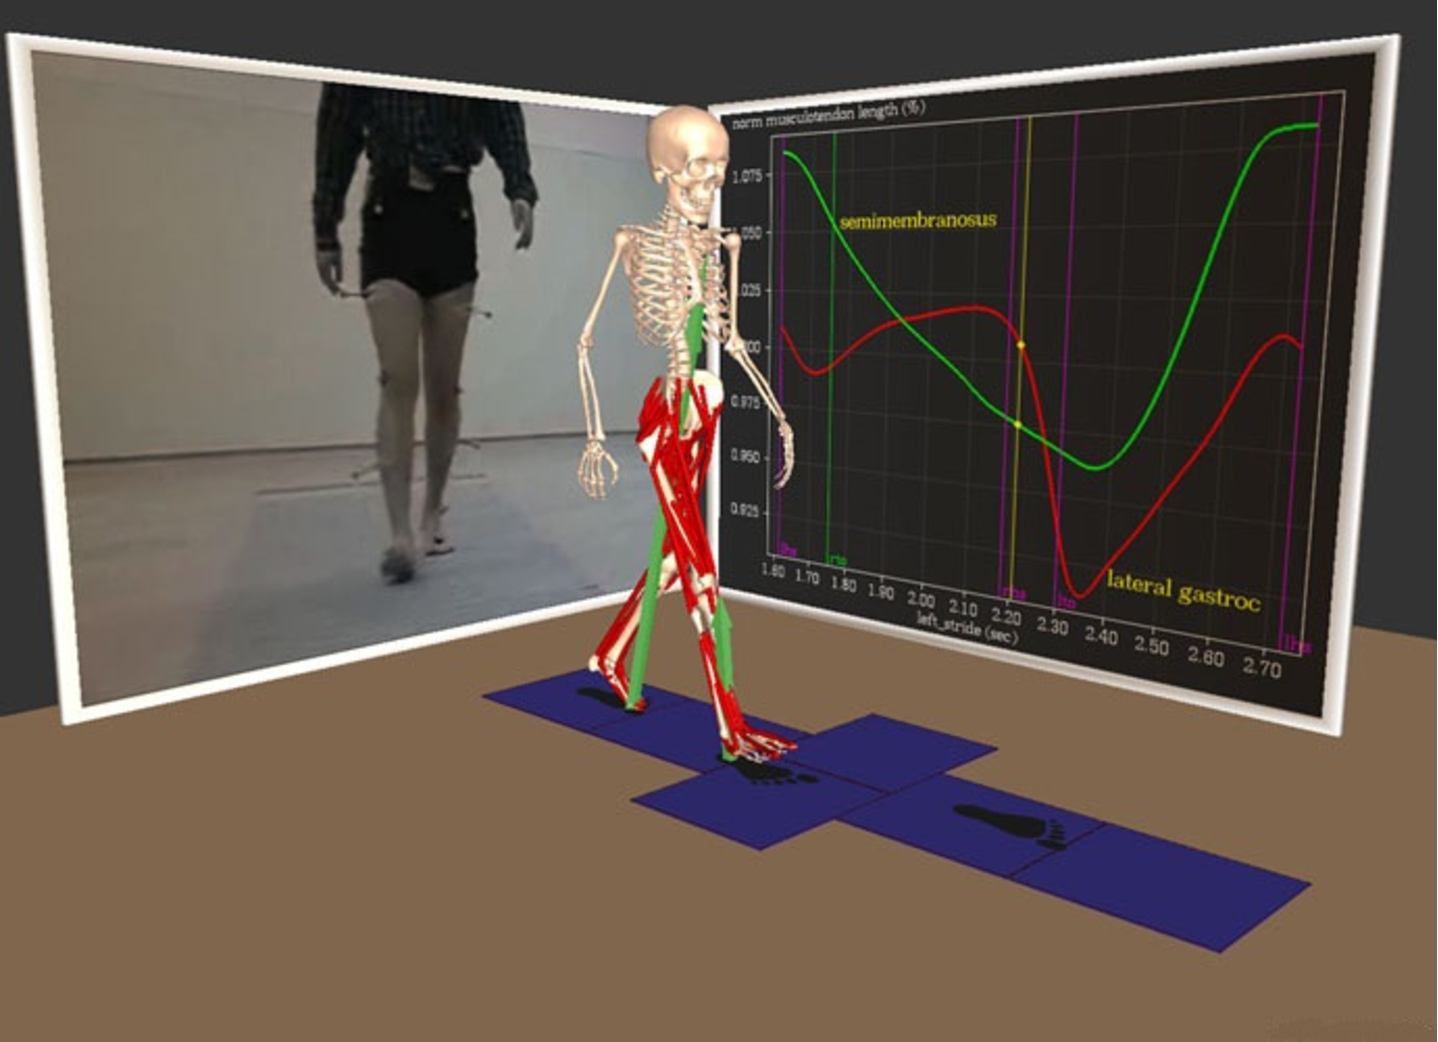
\includegraphics[width =0.25\linewidth,height=0.2\linewidth]{MotionModule.pdf}}
\subfloat[智能监控]{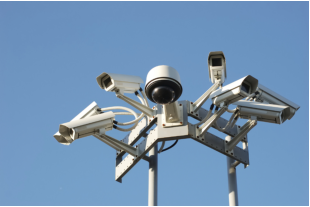
\includegraphics[width =0.25\linewidth,height=0.2\linewidth]{Surveillance.pdf}}
\caption{视觉跟踪的实际应用}
\label{fig:gen_applications}
\end{figure}
\end{frame}

%\begin{frame}{视觉跟踪中的挑战}

%一个良好的跟踪系统需要满足以下要求:

%\begin{block}{鲁棒性}

%鲁棒性意味着即使在复杂的条件下,跟踪算法也能够跟踪感兴趣的对象。跟踪困难可能是杂乱的背景、局部或整体光照变化、遮挡以及复杂的物体运动。
%\end{block}

%\begin{block}{适应性}

%除了对象所处环境的各种变化之外,对象本身也经历变化。这就需要跟踪系统对物体外观拥有稳定的适应机制。
%\end{block}

%\begin{block}{实时性}

%实时处理实时视频流的系统必须具有高处理速度。因此,除了高性能的算法,还需要快速和优化的实现。为了实现对于人眼而言的平滑的视频输出,必须建立至少每秒15帧的帧率。
%\end{block}

%\end{frame}
 
%\subsection{国内外研究现状}

%\begin{frame}{跟踪算法模型}

%\begin{block}{}
%自20世纪80年代以来,已有很多视觉跟踪算法提出。根据模型构建机制的不同,跟踪算法可以分为两类:生成式方法和判别式方法。生成式跟踪器通过搜索最佳匹配窗口执行跟踪,判别式方法依靠学习从背景中区分出目标。
%\end{block}

%\centering
%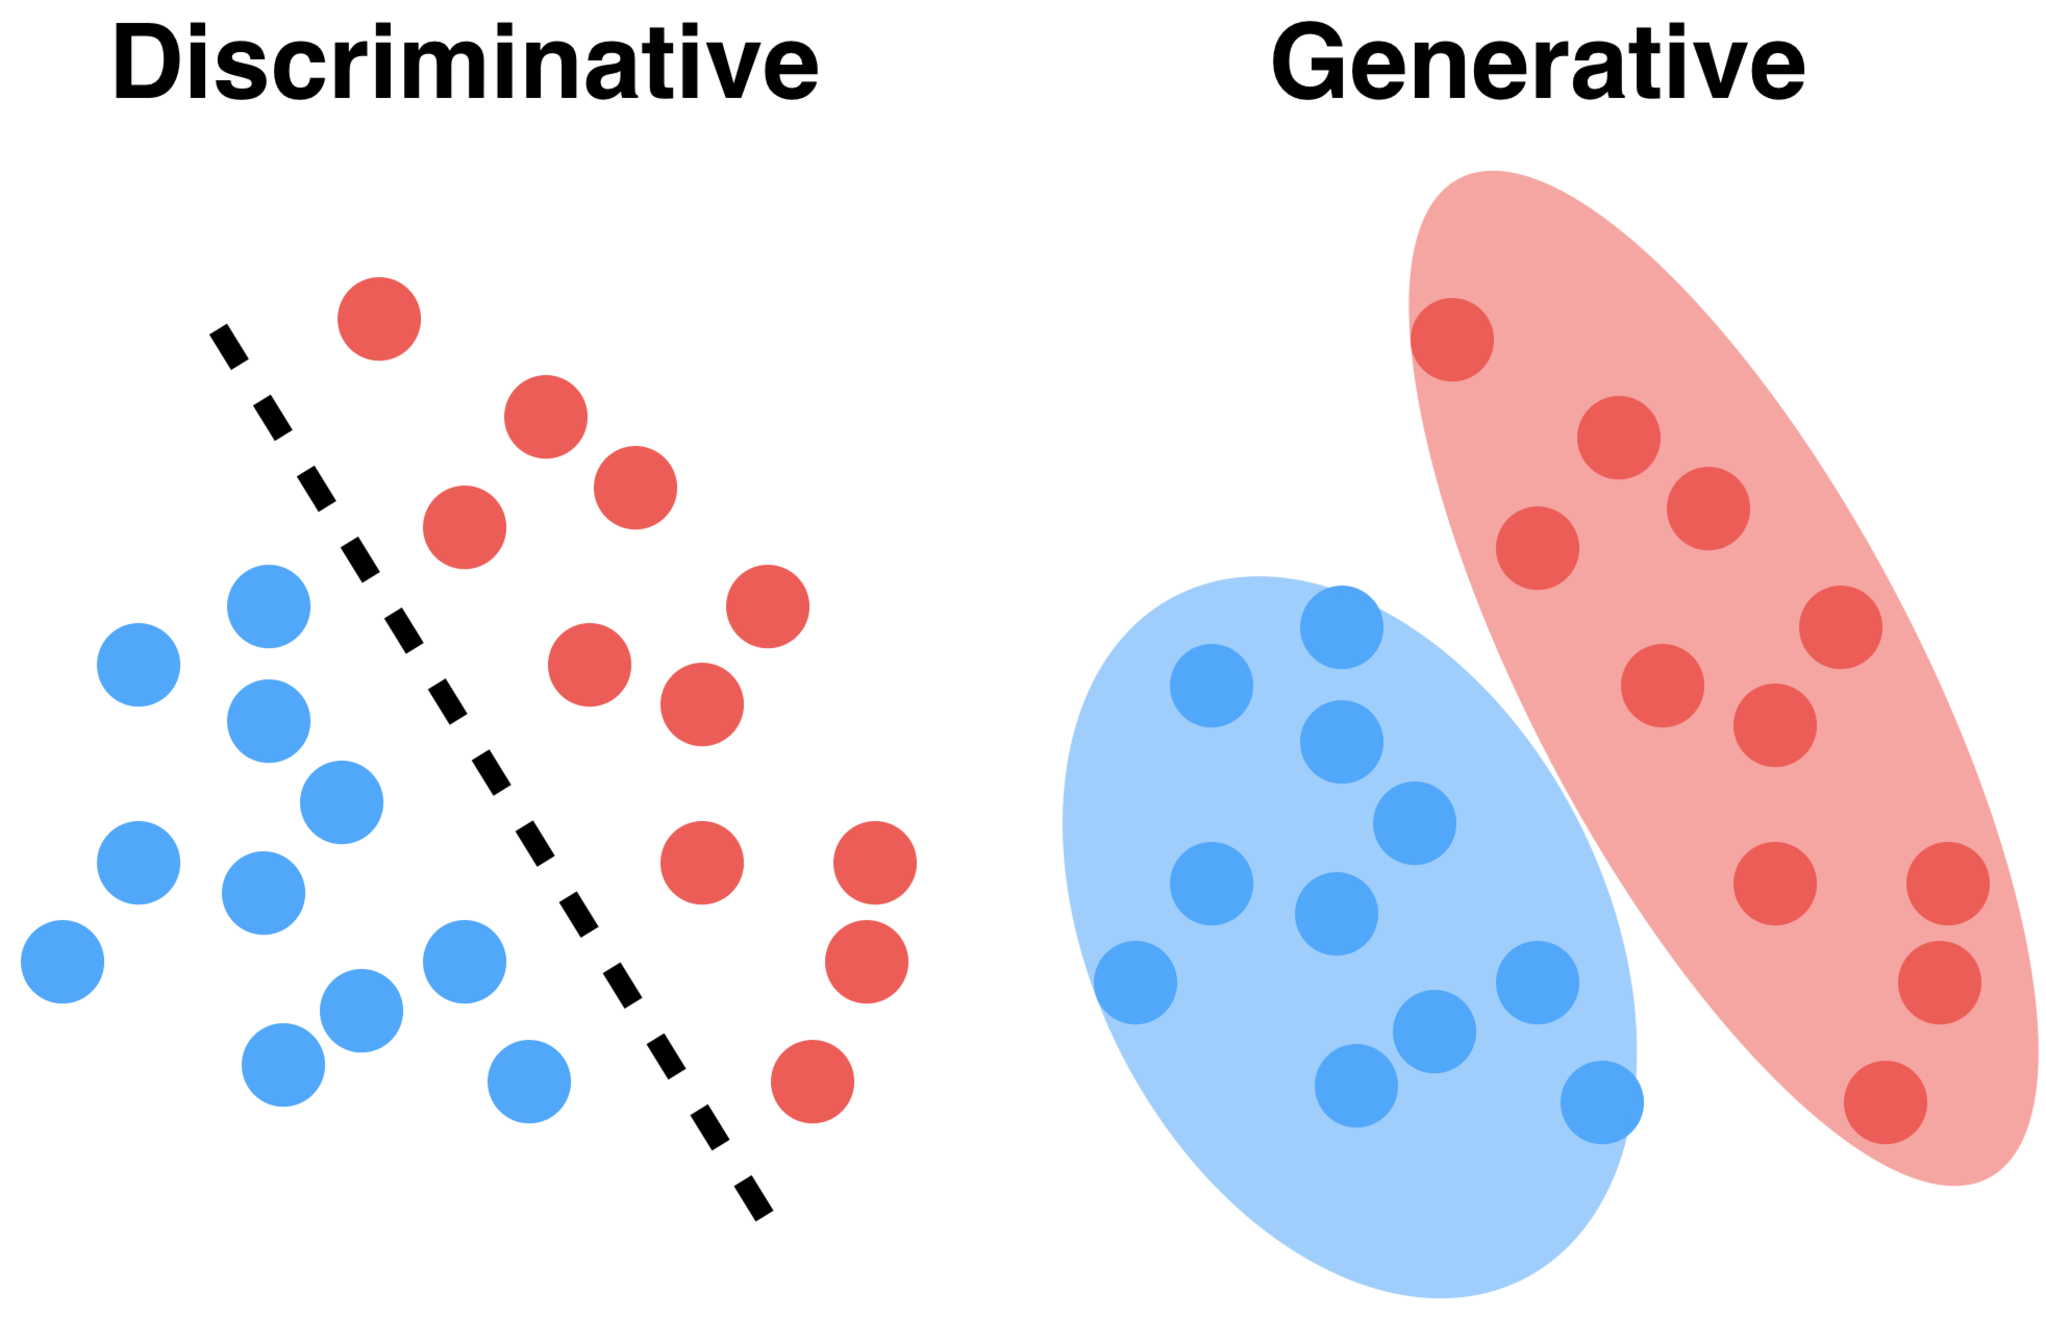
\includegraphics[width =0.5\textwidth,height =0.32\textwidth]{Discriminative_generative.pdf}

%\end{frame}


  \section{基于逻辑回归的集成学习跟踪}

\begin{frame}{工作点1}
    \tableofcontents[sections=\thesection]
\end{frame}

\subsection{算法简介}
\begin{frame}{算法简介}


\begin{block}{}
    基于逻辑回归的集成学习跟踪算法借助简单快速的弱分类器预测目标。为克服弱分类器的性能缺陷,以逻辑回归对其进行选取和集成。该算法以简单特征(Haar-like特征)和粗糙分类器为基础,并显著提高了跟踪的准确性。
    \end{block}
\end{frame}

\subsection{逻辑回归分类器}

\begin{frame}{逻辑回归}

\begin{center}
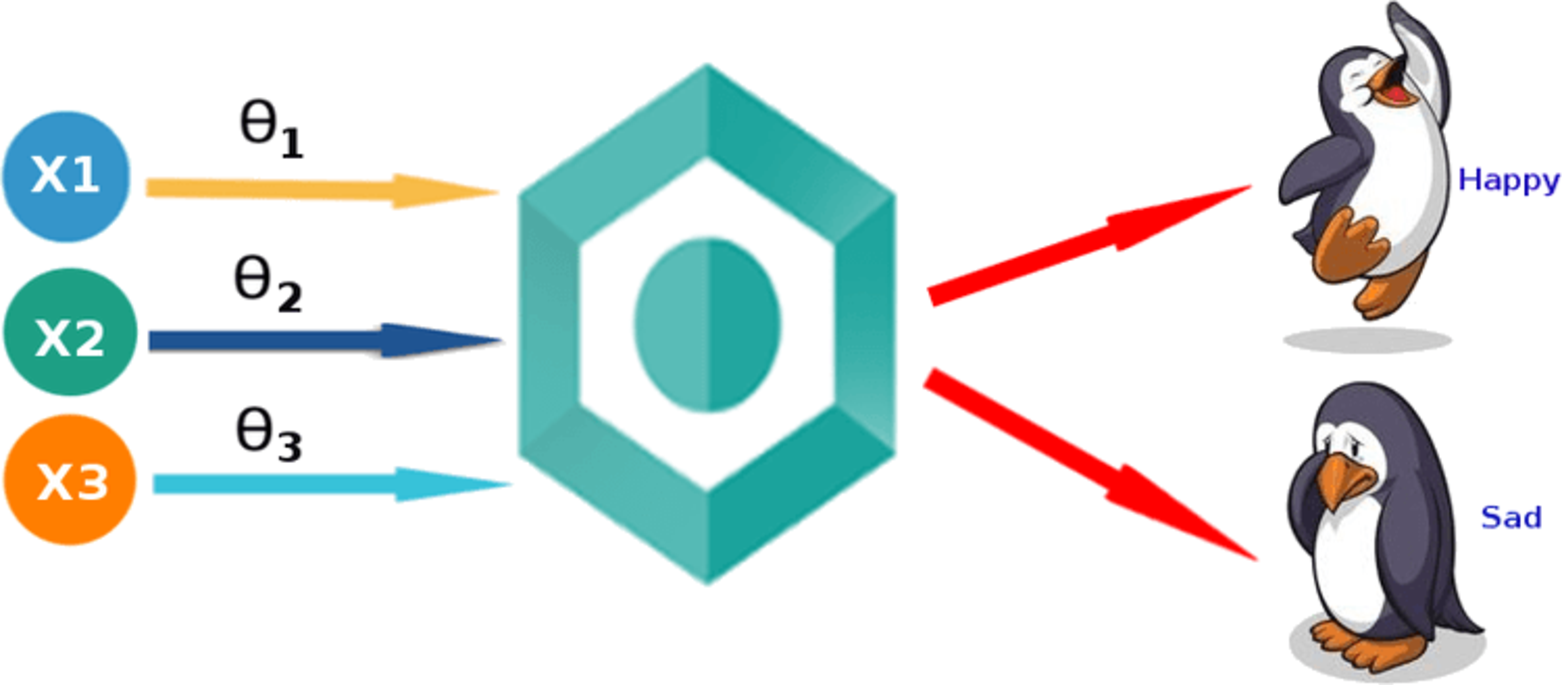
\includegraphics[width =0.5\textwidth,height =0.24\textwidth]{logisticregression.pdf}
\end{center}

逻辑回归为概率型非线性回归模型,是研究分类观察结果与影响因素之间关系的一种多变量分析方法。
~\\
\begin{equation}
P(y|x,w)=\frac{1}{1+\exp(-yx^{T}w) }
\label{eq:LR}
\end{equation}
~\\
其中$ x\in \mathbb{R}^{N} $为一组解释变量或者特征变量,$ y\in \{ -1,+1 \} $为相关联的二进制输出。

\end{frame}
\begin{frame}{模型参数}
逻辑回归试图寻找特征空间中的以法向量$ w\in \mathbb{R}^{N} $为参数的分类超平面,将样本分为两类。
假设给定一个训练或观测样本集合$ x=\{x_{1},x_{2},...,x_{M}\} $与其对应标签$ y=\{y_{1},y_{2},...,y_{M}\} $,模型参数w可通过样本的最大似然估计得到。最大似然估计函数最小化平均损失:
~\\
\begin{equation}
l_{avg}(w)=\frac{1}{M}\sum _{i=1}^{M} \log \left(1+\exp \left( -y_{i} w^{T}x_{i}\right)  \right)
\end{equation}
~\\
\end{frame}

\subsection{弱分类器}

\begin{frame}{Haar-like特征弱分类器}
本章算法使用Haar-like特征。每个弱分类器$ h_{k} $由1个 Haar-like特征$ f_{k} $ 和4个在线估计的参数$ (\mu_{+},\sigma_{+},\mu_{-},\sigma_{-}) $组成。分类器返回对数比值比:
\begin{equation}
\begin{aligned}
    h_{k}(x) &=\log[\frac{P(y=+1|f_{k}(x))}{P(y=-1|f_{k}(x))}]\\
          &=\log[\frac{P(f_{k}(x)|y=+1)P(y=+1)}{P(f_{k}(x)|y=-1)P(y=-1)}]
\end{aligned}
\end{equation}
其中$ P(f_{k}(x)|y=+1) $和$ P(f_{k}(x)|y=-1) $服从正态分布$ N(\mu_{+},\sigma_{+}) $。这里令$ P(y=+1)=P(y=-1) $,根据贝叶斯规则可以求解上述等式。
\end{frame}
\begin{frame}{弱分类器更新}
当弱分类器获得新数据时,使用如下方法进行更新:

\begin{equation}
\mu_{+}\longleftarrow \gamma\mu_{+}+(1-\gamma)\frac{1}{M}\sum_{i|y_{i}=+1}f_{k}(x_{i})
\label{eq:updatMuPosi}
\end{equation}
\begin{equation}
\mu_{-}\longleftarrow \gamma\mu_{-}+(1-\gamma)\frac{1}{M}\sum_{i|y_{i}=-1}f_{k}(x_{i})
\label{eq:updatMuNeg}
\end{equation}
\begin{equation}
\sigma_{+}\longleftarrow \gamma\log\sigma_{+}+(1-\gamma)\sqrt{\frac{1}{M}\sum_{i|y_{i}=+1}(f_{k}(x_{i})-\mu_{+})^{2}}
\label{eq:updatSigmaPosi}
\end{equation}
\begin{equation}
\sigma_{-}\longleftarrow \gamma\log\sigma_{-}+(1-\gamma)\sqrt{\frac{1}{M}\sum_{i|y_{i}=-1}(f_{k}(x_{i})-\mu_{-})^{2}}
\label{eq:updatSigmaNeg}
\end{equation}

\end{frame}

\subsection{逻辑回归集成学习框架}

\begin{frame}{跟踪流程}
\begin{figure}[htbp]
  \centering
  % Requires \usepackage{graphicx}
  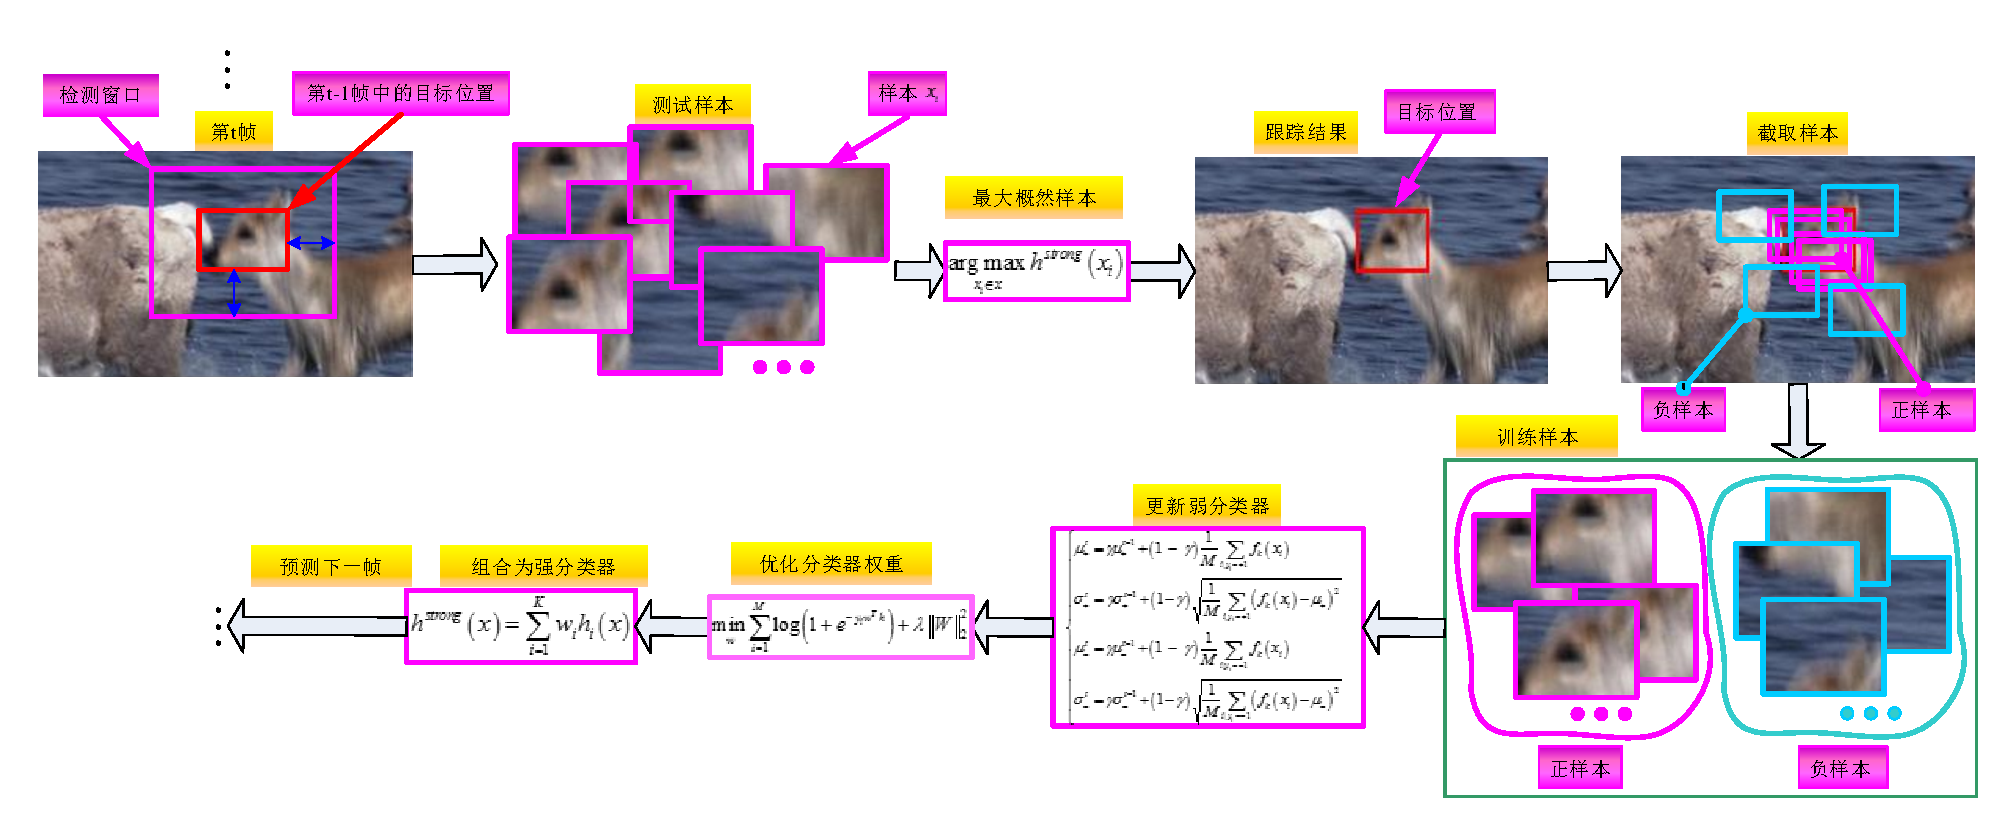
\includegraphics[width=\linewidth]{figures/LR_ArchitecturalStructure.pdf}\\
\caption{逻辑回归集成学习跟踪模型}
\label{fig:LR_ArchitecturalStructure}
\end{figure}

\end{frame}

%\begin{frame}{强分类器预测目标位置}
%当新一帧到来时,算法根据前一帧位置设定测试区域,从中分割出图像块集合。Boosting分类器给出每个图像块是目标的概率值,将概率值最高的图像块认定为目标。
%~\\
%\begin{equation}
%h^{strong}(x)= \sum _{i=1}^{K} w_{i}h_{i}(x)=w^{T}h(x)
%\label{eq:strongClassification}
%\end{equation}
%~\\
%其中$ h_{i}(x),i=1,2,...,K $是弱分类器集合中挑选出的性能较好的K个弱分类器。
%\end{frame}

%\begin{frame}{优化弱分类器权重}
%根据目标位置可以分割出若干图像块作为正负训练样本。在算法中,每一个图像块被视为一个训练样本,并对应一个特征向量。逻辑回归挑选出较好的分类器并赋予合适的权重:
%~\\
 %\begin{equation}
 %\min_{w}\sum _{i=1}^{M} \log \left(1+\exp \left( -y_{i} w^{T}h(x_{i})\right) \right) + \lambda ||w||^{2}_{2}
%\label{eq:optimizeW}
%\end{equation}
%~\\
%其中,$ h(x) = [h_1(x) , h_2(x) , \dots , h_N(x)] $。公式(\ref{eq:optimizeW})通过减少预测标签和真实标签之间的总误差确定弱分类器的权重。

%\end{frame}

\subsection{实验结果}

\begin{frame}{中心位置误差(CLE)}

\begin{table}[!t]
\centering
\renewcommand{\arraystretch}{1.5}
\caption{中心位置误差(像素)}

\begin{adjustbox}{max width=\textwidth}
\begin{tabular}{|c|c|c|c|c|c|c|c|c|c|}
\hline Sequence & CT & CXT & DF & MIL & SCM & Struck & TLD & VTD & Ours\\
\hline Basketball & 89  & 215 & 18 & 92 & 53 & 118 & 269 & \textcolor{red}{6}  & \textcolor{blue}{10} \\
\hline David3     & 89  & 222 & 51 & \textcolor{blue}{30} & 73 & 107 & 281 & 67 & \textcolor{red}{13} \\
\hline Football   & \textcolor{blue}{12}  & 13  & \textcolor{red}{9}  & \textcolor{blue}{12} & 17 & 17  & 14  & 14 & \textcolor{blue}{12} \\
\hline Jogging    & 92  & \textcolor{blue}{6}   & 31 & 96 & 132& 62  & 7   & 83 &  \textcolor{red}{5}\\
\hline Liquor     & 186 & 132 & 221& 142& 99 & 91  & 100 & \textcolor{blue}{60} & \textcolor{red}{57} \\
\hline
\end{tabular}
\end{adjustbox}
\label{tab:LR_CLE}
\end{table}

中心位置误差(Center Location Error, CLE),即检测到的目标框中心与真实目标框中心的平均欧式距离,其值越小代表跟踪结果准确性越高。
\end{frame}

\begin{frame}{重叠精度(OP)}

\begin{table}[!t]
\centering
\renewcommand{\arraystretch}{1.5}
\caption{阈值为0.5的重叠精度(\%)}

\begin{adjustbox}{max width=\textwidth}
\begin{tabular}{|c|c|c|c|c|c|c|c|c|c|}
\hline Sequence & CT & CXT & DF & MIL & SCM & Struck & TLD & VTD & Ours\\
\hline Basketball & 25.93  & 2.48 & 71.59 & 27.45 & 60.28 & 10.21 & 2.48 & \textcolor{red}{92.41}  & \textcolor{blue}{81.51} \\
\hline David3     & 34.92  & 13.89 & \textcolor{blue}{74.21} & 68.25 & 48.02 & 33.73 & 10.32 & 48.41 & \textcolor{red}{84.52} \\
\hline Football   & 78.45 & 65.19  & \textcolor{red}{84.25}  & 73.76 & 57.18 & 66.02  & 41.16  & 76.80 & \textcolor{blue}{78.72} \\
\hline Jogging    & 22.48  & \textcolor{blue}{95.44}   & 21.50 & 22.48 & 21.17& 22.48  & \textcolor{red}{96.74}   & 21.50 &  {95.11}\\
\hline Liquor     & 20.85 & 20.96 & 22.92& 20.10& 32.45 & 40.61  & 56.17 & \textcolor{blue}{57.96} & \textcolor{red}{69.79} \\
\hline
\end{tabular}
\end{adjustbox}
\label{tab:LR_OP}
\end{table}

阈值为0.5的重叠精度(Overlap Precision, OP),即所得目标边界框与真实边界框重叠率超过给定阈值的帧数占总视频的百分比(本文实验中阈值为0.5),其值越大代表跟踪结果越好。
\end{frame}

\newcommand{\mycline}[1]{\tikz{\draw[#1 , line width=3] (0,0) -- (.2,0);}}
\begin{frame}{代表性序列帧及对比算法跟踪结果}

\begin{figure}[htp]
	
	\centering
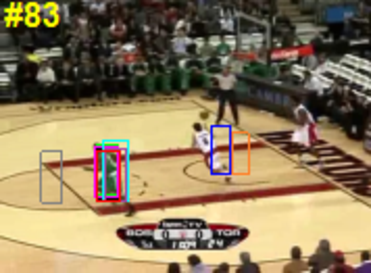
\includegraphics[width=0.31\textheight,height=0.25\textheight]{figures/Figure2a1.pdf}
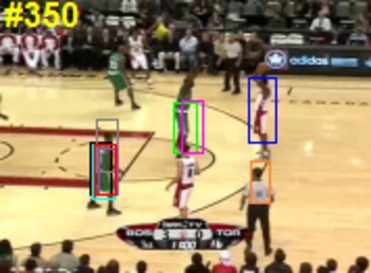
\includegraphics[width=0.31\textheight,height=0.25\textheight]{figures/Figure2a2.pdf}
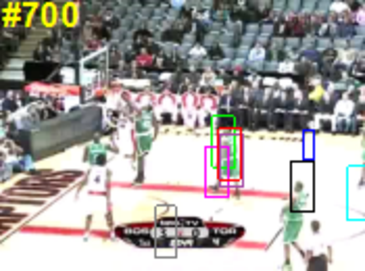
\includegraphics[width=0.31\textheight,height=0.25\textheight]{figures/Figure2a3.pdf}\\

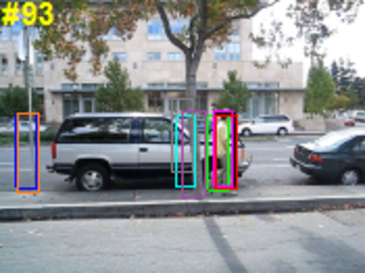
\includegraphics[width=0.31\textheight,height=0.25\textheight]{figures/Figure2b1.pdf}
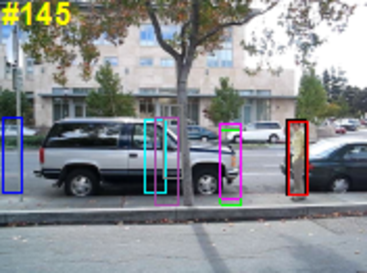
\includegraphics[width=0.31\textheight,height=0.25\textheight]{figures/Figure2b2.pdf}
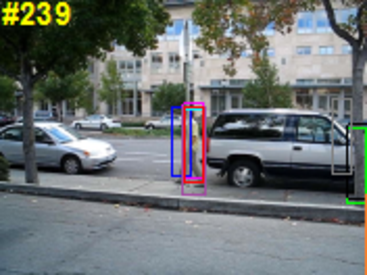
\includegraphics[width=0.31\textheight,height=0.25\textheight]{figures/Figure2b3.pdf}\\

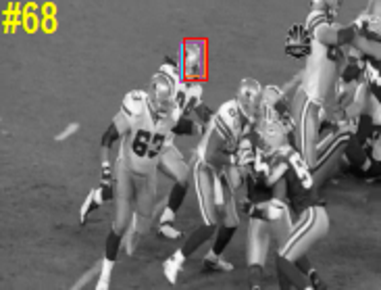
\includegraphics[width=0.31\textheight,height=0.25\textheight]{figures/Figure2c1.pdf}
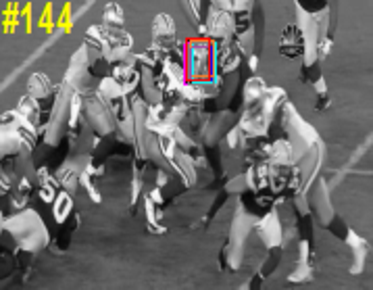
\includegraphics[width=0.31\textheight,height=0.25\textheight]{figures/Figure2c2.pdf}
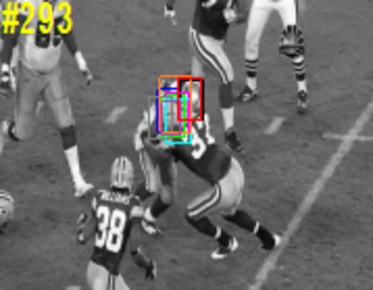
\includegraphics[width=0.31\textheight,height=0.25\textheight]{figures/Figure2c3.pdf}\\

   \mycline{green}CT
   \mycline{blue}CXT
   \mycline{black}DT
   \mycline{pink}MIL
   \mycline{cyan}SCM
   \mycline{gray}Struck
   \mycline{orange}TLD
   \mycline{purple}VTD
   \mycline{red}Ours

%\caption{跟踪过程中代表性序列帧及对比算法跟踪结果}
%\label{fig:LR_trackingResultSample}
\end{figure}

\end{frame}

\begin{frame}{代表性序列帧及对比算法跟踪结果}

\begin{figure}[htp]
	
	\centering
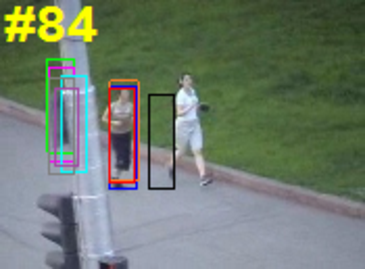
\includegraphics[width=0.31\textheight,height=0.25\textheight]{figures/Figure2d1.pdf}
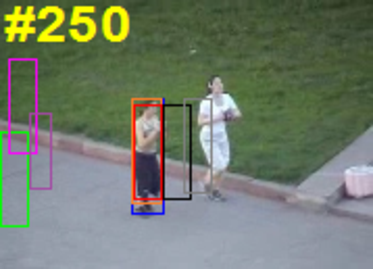
\includegraphics[width=0.31\textheight,height=0.25\textheight]{figures/Figure2d2.pdf}
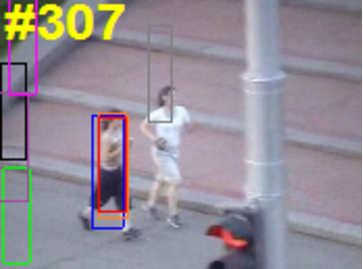
\includegraphics[width=0.31\textheight,height=0.25\textheight]{figures/Figure2d3.pdf}\\

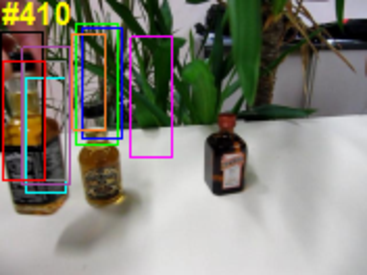
\includegraphics[width=0.31\textheight,height=0.25\textheight]{figures/Figure2e1.pdf}
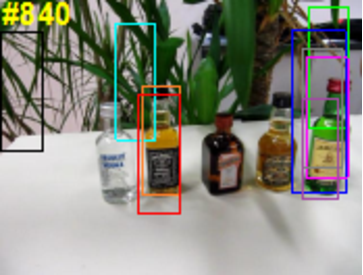
\includegraphics[width=0.31\textheight,height=0.25\textheight]{figures/Figure2e2.pdf}
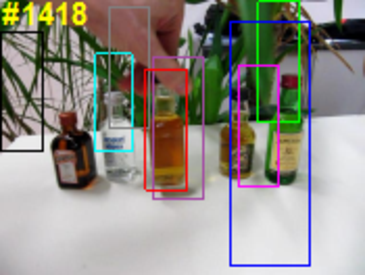
\includegraphics[width=0.31\textheight,height=0.25\textheight]{figures/Figure2e3.pdf}\\

   \mycline{green}CT
   \mycline{blue}CXT
   \mycline{black}DT
   \mycline{pink}MIL
   \mycline{cyan}SCM
   \mycline{gray}Struck
   \mycline{orange}TLD
   \mycline{purple}VTD
   \mycline{red}Ours

%\caption{跟踪过程中代表性序列帧及对比算法跟踪结果}
%\label{fig:LR_trackingResultSample}
\end{figure}

\end{frame}




  \include{sections/CorrelationFilter}
  \section{结构化输出的相关滤波跟踪}

\begin{frame}{工作点3}
    \tableofcontents[sections=\thesection]
\end{frame}

\subsection{算法简介}
\begin{frame}{算法简介}

\begin{block}{着眼问题}
相关滤波器利用傅里叶域特性能够高效地预测,但边界效应对跟踪性能有显著的影响。
\end{block}

\begin{block}{解决方案}
本章提出一种结构化输出的相关滤波跟踪方法,在利用相关滤波密集取样优势的同时,显著减少边界效应带来的性能损失。
\end{block}
\end{frame}


\subsection{有限边界的相关滤波器}

\begin{frame}{MOSSE相关滤波器}
MOSSE相关滤波器可以在空间域中表示为求解岭回归问题:
~\\
\begin{equation}
    E(h)= \frac{1}{2}\sum_{i=1}^N\sum_{j=1}^D\|y_i(j)-h^\top x_i[\Delta\tau_j]\|_2^2 + \frac{\lambda}{2}\|h\|_2^2
    \label{eq:CFwLB_MOSSEinSpatial}
\end{equation}
~\\
其中$y_i\in \mathbb{R}^D$是第$i$个观测$x_i\in \mathbb{R}^D$的期望响应,$\lambda$是正则项参数。$\mathbb{C} = [\Delta\tau_1,\dots,\Delta\tau_D]$表示长度为$D$的信号的所有循环移位集合。
\end{frame}

\begin{frame}{边界效应}

\begin{columns}
\centering
\column{0.7\linewidth}
\setlength{\parindent}{2\ccwd}

相关滤波器从由1个真实示例与其他合成示例组成的非平衡集合中估计出判别性模板。这些合成的样本是通过对真实样本应用循环移位来创建的。

~\\
如右图所示,循环移位的样本都受循环边界效应的影响,并不能代表真实的移动。边界效应可以显著影响所得到的估计模板,使得相关滤波器对平移中的偏差特别敏感。

\column{0.3\textwidth}
   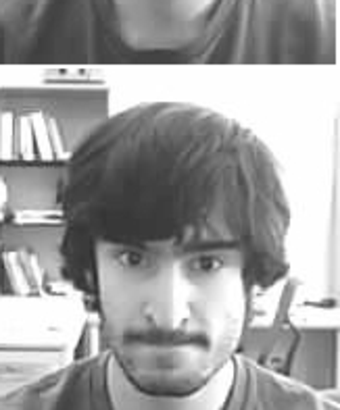
\includegraphics[width =\textwidth,height =1.3\textwidth]{CFwLB_a_3.pdf}
\end{columns} 
\end{frame}

\begin{frame}{引入掩蔽矩阵}
%%Boundary Effects

\begin{columns}
\centering
\column{0.65\textwidth}
\setlength{\parindent}{2\ccwd}

    有限边界滤波器能够在空间上避免边界效应。其训练信号$x\in \mathbb{R}^T$的大小比滤波器$h\in\mathbb{R}^D$大。通过使用掩蔽矩阵$P\in \mathbb{R}^{D\times T}$,可以将等式(\ref{eq:CFwLB_MOSSEinSpatial})表示为:
\column{0.3\linewidth}
   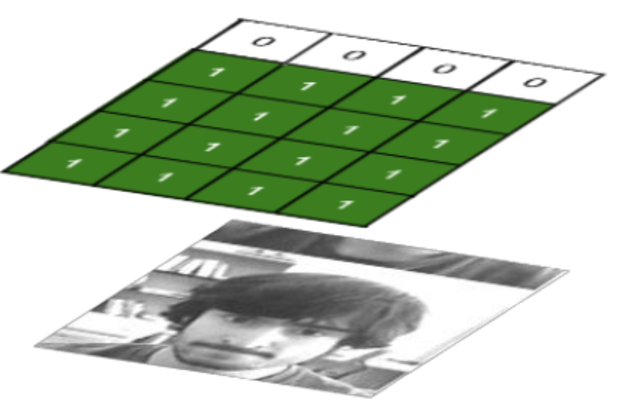
\includegraphics[width =\textwidth,height =0.7\textwidth]{MaskingMatrix.pdf}
\end{columns} 
~\\
\begin{equation}
    E(h)= \frac{1}{2}\sum_{i=1}^N\sum_{j=1}^T\|y_i(j)-h^\top Px_i[\Delta\tau_j]\|_2^2 + \frac{\lambda}{2}\|h\|_2^2
    \label{eq:CFwLB_MOSSEinSpatialwithMaskingMatix}
\end{equation}
~\\
掩蔽矩阵$P$封装了信号,其中的1和0决定哪一部分应该是有效的,哪一部分是无效的。

\end{frame}

\begin{frame}{样本对比}
\begin{figure}[htp]
\centering
\subfloat[传统滤波器样本]{
                          \begin{minipage}[b]{0.4\linewidth}
                          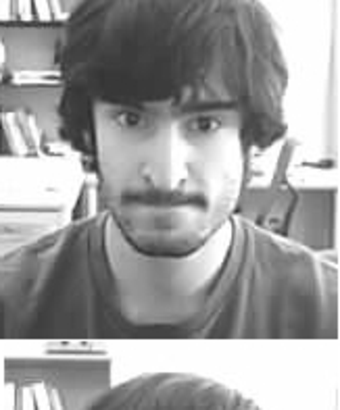
\includegraphics[width =0.3\linewidth,height =0.4\linewidth]{CFwLB_a_2.pdf}
                          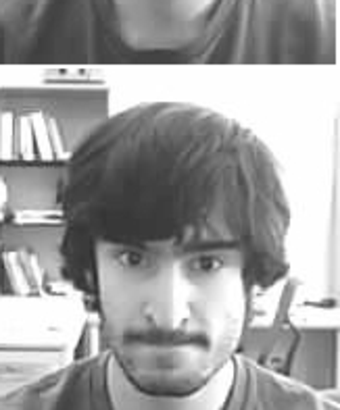
\includegraphics[width =0.3\linewidth,height =0.4\linewidth]{CFwLB_a_3.pdf}
                          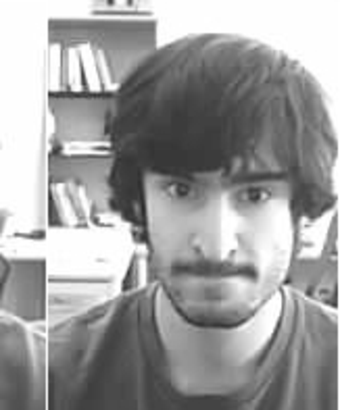
\includegraphics[width =0.3\linewidth,height =0.4\linewidth]{CFwLB_a_4.pdf}\\
                          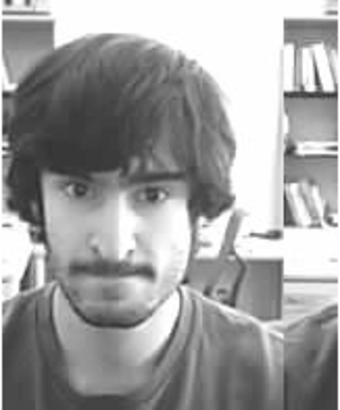
\includegraphics[width =0.3\linewidth,height =0.4\linewidth]{CFwLB_a_5.pdf}
                          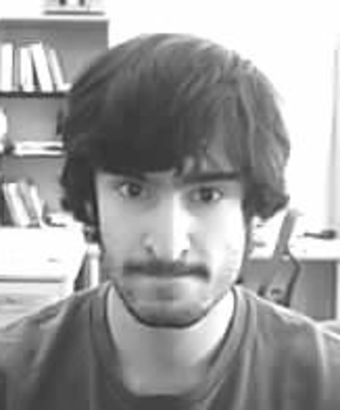
\includegraphics[width =0.3\linewidth,height =0.4\linewidth]{CFwLB_a_1.pdf}
                          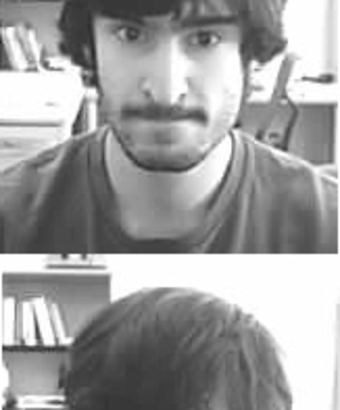
\includegraphics[width =0.3\linewidth,height =0.4\linewidth]{CFwLB_a_6.pdf}\\
                          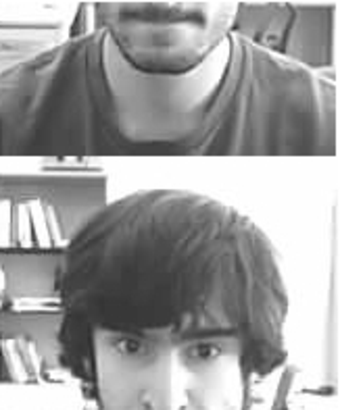
\includegraphics[width =0.3\linewidth,height =0.4\linewidth]{CFwLB_a_7.pdf}
                          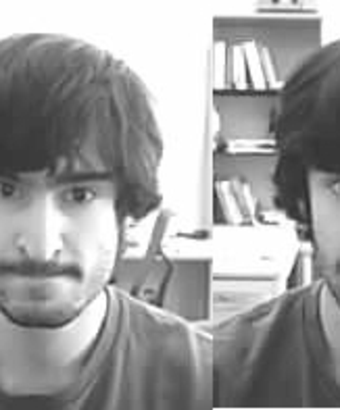
\includegraphics[width =0.3\linewidth,height =0.4\linewidth]{CFwLB_a_8.pdf}
                          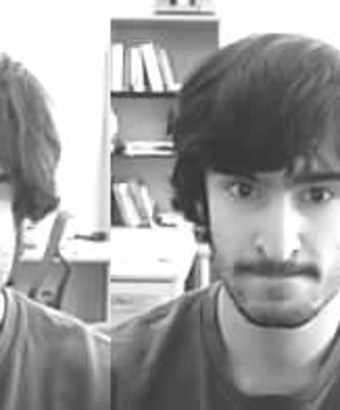
\includegraphics[width =0.3\linewidth,height =0.4\linewidth]{CFwLB_a_9.pdf}
                          \end{minipage}

\label{fig:CFwLB_CFSamples}}
\subfloat[有限边界滤波器样本]{
                              \begin{minipage}[b]{0.3\linewidth}
                              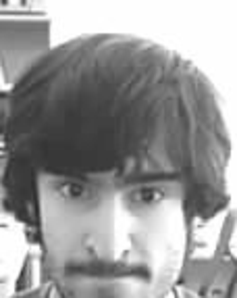
\includegraphics[width =0.3\linewidth,height =0.4\linewidth]{CFwLB_b_2.pdf}
                              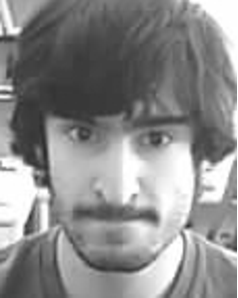
\includegraphics[width =0.3\linewidth,height =0.4\linewidth]{CFwLB_b_3.pdf}
                              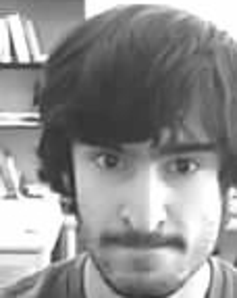
\includegraphics[width =0.3\linewidth,height =0.4\linewidth]{CFwLB_b_4.pdf}\\
                              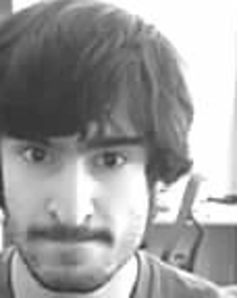
\includegraphics[width =0.3\linewidth,height =0.4\linewidth]{CFwLB_b_5.pdf}
                              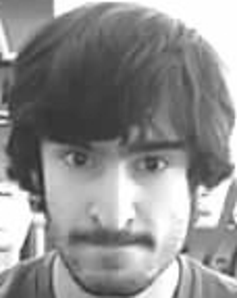
\includegraphics[width =0.3\linewidth,height =0.4\linewidth]{CFwLB_b_1.pdf}
                              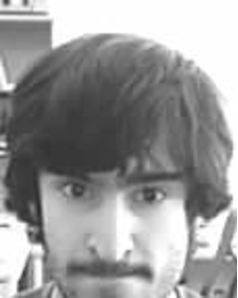
\includegraphics[width =0.3\linewidth,height =0.4\linewidth]{CFwLB_b_6.pdf}\\
                              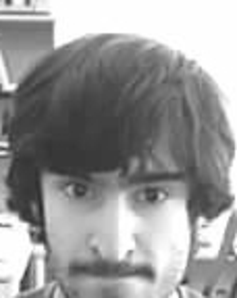
\includegraphics[width =0.3\linewidth,height =0.4\linewidth]{CFwLB_b_7.pdf}
                              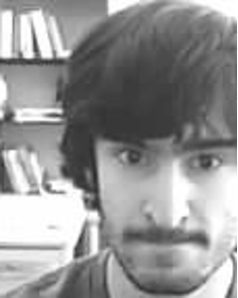
\includegraphics[width =0.3\linewidth,height =0.4\linewidth]{CFwLB_b_8.pdf}
                              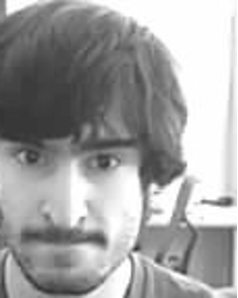
\includegraphics[width =0.3\linewidth,height =0.4\linewidth]{CFwLB_b_9.pdf}\\
                              \end{minipage}

\label{fig:CFwLB_Samples}}
\caption{有限边界滤波器}
\label{fig:CFwLB_Intro}
\end{figure}
\end{frame}

%\begin{frame}{滤波器的傅里叶域表示}
%等式(\ref{eq:CFwLB_MOSSEinSpatialwithMaskingMatix})可以在傅立叶域中表示为:
%~\\
%\begin{equation}
%E(h)= \frac{1}{2}\sum_{i=1}^N\sum_{j=1}^T\|\hat{y}_i(j)-\mathrm{diag}(\hat{x}_i)^\top\sqrt{D}FP^\top h]\|_2^2 + \frac{\lambda}{2}\|h\|_2^2
    %\label{eq:CFwLB_MOSSEwithMaskingMatixInFourier}
%\end{equation}
%~\\
%\end{frame}

%\begin{frame}{增强拉格朗日方法(ALM)}
%引入辅助变量$g$,等式(\ref{eq:CFwLB_MOSSEwithMaskingMatixInFourier})可以相同地表示为:
%~\\
%\begin{equation}
%\begin{aligned}
%E(h,\hat{g})& = \frac{1}{2}\sum_{i=1}^N\sum_{j=1}^T\|\hat{y}_i(j)-\mathrm{diag}(\hat{x}_i)^\top \hat{g}]\|_2^2 + \frac{\lambda}{2}\|h\|_2^2 \\
    %\mathrm{s.t.}\quad &\hat{g}= \sqrt{D}FP^\top h
    %\end{aligned}
    %\label{eq:CFwLB_objectiveFunction}
%\end{equation}
%~\\
%可以通过增强拉格朗日方法(Augmented Lagrange Method, ALM)来处理引入的等式约束。
%\end{frame}

%\begin{frame}{目标函数的ALM的表示}
%~\\
%\begin{equation}
%\begin{aligned}
%\mathcal{L}(\hat{g},h,\hat{\zeta})= &\frac{1}{2}\sum_{i=1}^N\|\hat{y}_i(j)-\mathrm{diag}(\hat{x}_i)^\top \hat{g}]\|_2^2 + \frac{\lambda}{2}\|h\|_2^2\\
                                    %&+ \hat{\zeta}^\top(\hat{g}-\sqrt{D}FP^\top h)\\
                                    %&+ \frac{\mu}{2}\|\hat{g}-\sqrt{D}FP^\top h\|_2^2
%\end{aligned}
    %\label{eq:CFwLB_augmented LagrangianObjectiveFunction}
%\end{equation}
%~\\
%其中$\mu$是控制ALM收敛速率的惩罚因子,$\hat{\zeta}$是在等式(\ref{eq:CFwLB_objectiveFunction})中强制引入的等式约束所需拉格朗日矢量的傅里叶变换。
%\end{frame}

\subsection{对于有限边界滤波器的改进}

\begin{frame}{标签图}
\begin{columns}
\centering
\column{0.4\textwidth}
\begin{figure}[htp]
  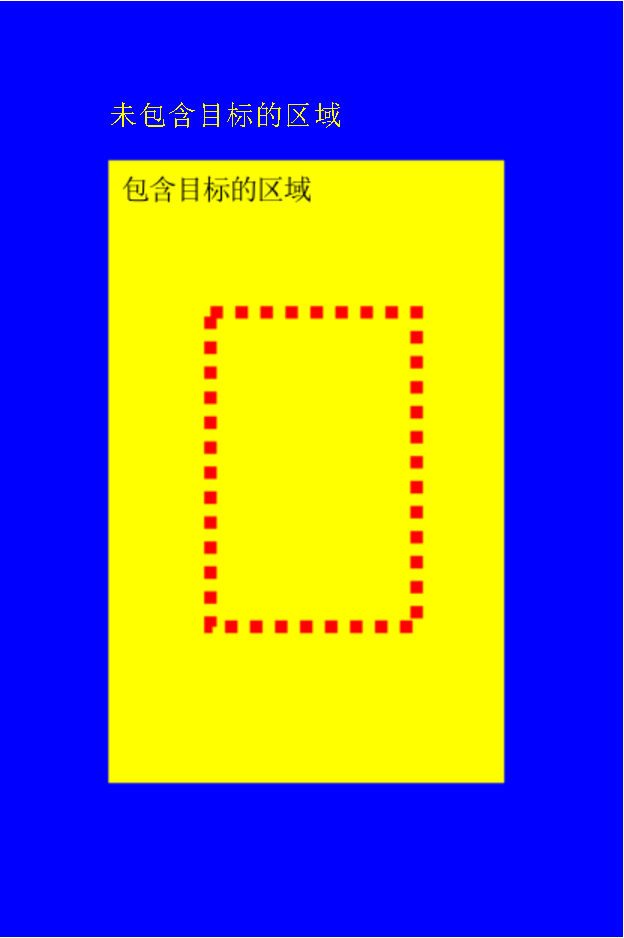
\includegraphics[height=.7\textheight]{figures/CFwLBlabels.pdf}
\caption{有限边界滤波器标签图}
\label{fig:CFwLB_labels}
\end{figure}

\column{0.6\textwidth}
\setlength{\parindent}{2\ccwd}

有限边界相关滤波器只对样本进行了加工,而未注意到样本与标签的匹配问题。由于扩大滤波器尺寸的同时仍采用了传统相关滤波器的平滑高斯函数生成标签,未包含目标的样本块同样被赋予了正标签。因而,滤波器无法学习到区分度高的特征。
\end{columns}
\end{frame}

\begin{frame}{以结构化方式定义样本}

借鉴图像检测中的结构化输出方法,以样本框的坐标作为样本标签,这使得样本描述与实际问题相一致。
~\\
\begin{equation}
E(h)= \frac{1}{2}\sum_{i=1}^N\sum_{j=1}^T\|\widehat{l(y_i(j))}-\mathrm{diag}(\hat{x}_i)^\top\sqrt{D}FP^\top h]\|_2^2 + \frac{\lambda}{2}\|h\|_2^2
    \label{eq:CFwLB_MOSSEwithMaskingMatixInFourierStructuredOutput}
\end{equation}
~\\
其中,评价函数$l(y)=\frac{\mathrm{Area}(y_i\cap y^\ast)}{\mathrm{Area}(y_i\cup y^\ast)}$表示样本框与目标框的重叠率,$y^\ast$为目标框的坐标表示,$\mathrm{Area}$表示求两个矩形框的面积。
\end{frame}

\subsection{实验结果}



%%%单元格中显示多行
\begin{frame}{距离精度(DP)}
\begin{table}[!t]
\centering
%%%增大行距
\renewcommand{\arraystretch}{1.3}
%\setlength{\abovecaptionskip}{15pt plus 3pt minus 2pt}
\captionsetup{belowskip=2pt,aboveskip=4pt}

\caption{20个像素偏差内的距离精度}
\begin{adjustbox}{max width=\textwidth}
    \begin{tabular}{|c|c|c|c|c|c|c|c|c|}
        \hline
        Sequance  & Frag  &  OAB  &  SBT  &  MIL  & Struck & CSK   & CFwLB   &  Ours \\ \hline
        
        Coke      & 0.034 & 0.168 & 0.048  & 0.117 & \textcolor{blue}{0.942} & 0.739 & 0.918   & \textcolor{red}{0.959}  \\ \hline
        David     & 0.121 & 0.151 & 0.204  & 0.229 & \textcolor{blue}{0.236} & \textcolor{blue}{0.236} & 0.144   & \textcolor{red}{0.396} \\ \hline
        Dog       & 0.173 & 0.157 & 0.079  & 0.197 & 0.157 & 0.144 & \textcolor{blue}{0.858}   & \textcolor{red}{0.992}  \\ \hline
        Doll      & 0.663 & 0.663 & 0.149  & 0.433 & 0.688 & 0.218 & \textcolor{blue}{0.947}& \textcolor{red}{ 0.986} \\ \hline
        Gym       & \textcolor{blue}{0.369} & 0.016 & 0.046  & 0.329 & 0.219 & 0.091 & 0.113   & \textcolor{red}{0.801}  \\ \hline
        KiteSurf  & 0.143 & 0.381 & 0.369  & 0.381 & \textcolor{blue}{0.905} & 0.321 & 0.274   & \textcolor{red}{0.964}  \\ \hline
        Surfer    & 0.176 & 0.045 & 0.133  & 0.088 & 0.157 & 0.005  & \textcolor{blue}{0.468}   & \textcolor{red}{0.997}  \\ \hline
    Sylvester     & 0.685 & 0.680 & 0.430  & 0.546 & \textcolor{blue}{0.929} & 0.717 & 0.921 & \textcolor{red}{0.947}\\ \hline
        Vase      & 0.166 & 0.155 & 0.129  & 0.166 & 0.140 & 0.166  & \textcolor{blue}{0.181}   & \textcolor{red}{0.657}  \\ \hline \hline

        mean      &0.281  & 0.268 & 0.176  & 0.276 & 0.486 & 0.293  & \textcolor{blue}{0.536}& \textcolor{red}{0.855} \\ \hline
\end{tabular}
\end{adjustbox}
\label{tab:CFwLB_precision}
\end{table}
\end{frame}

\begin{frame}{中心位置误差(CLE)}
\begin{table}[htbp]
\centering
\renewcommand{\arraystretch}{1.3}
\captionsetup{belowskip=2pt,aboveskip=4pt}

\caption{平均中心位置误差}
\begin{adjustbox}{max width=\textwidth}
    \begin{tabular}{|c|c|c|c|c|c|c|c|c|}
        \hline
        Sequance  & Frag  &  OAB  &  SBT  &  MIL  & Struck & CSK   & CFwLB   &  Ours \\ \hline
        
        Coke      & 124.8 & 35.9  & 365.3 & 46.7  &  \textcolor{red}{12.1}  & 13.6  & 13.2   &   \textcolor{blue}{12.9}  \\ \hline
        David     & 82.1  & 21.7  & 47.1  & \textcolor{red}{16.9}  & 42.8   &  \textcolor{blue}{17.7} & 73.6   &   28.9  \\ \hline
        Dog       & 12.2  & 10.7  & 172.5 & 8.2   &  10.4  &  \textcolor{blue}{7.0}  & 11.8   & \textcolor{red}{6.8}  \\ \hline
        Doll      & 13.7  & 12.4  & 113.9 & 16.7  & \textcolor{blue}{8.9}&  44.7 & 9.5    & \textcolor{red}{ 4.6} \\ \hline
        Gym       & 10.0  & 111.0 & 230.4 & 11.8  & 18.5   &  27.1 & \textcolor{blue}{9.5}  & \textcolor{red}{ 4.6} \\ \hline
        KiteSurf  & 141.1 & 64.6  & 32.9  & 22.6  & \textcolor{red}{6.1}   &  36.5 & 85.7    & \textcolor{blue}{10.6} \\ \hline
        Surfer    & 51.6  & 72.1  & 218.5 & 17.0  &\textcolor{blue}{9.0}   & 161.7 & 25.3    & \textcolor{red}{6.5} \\ \hline
        Sylvester & 15.0  & 14.8  & 101.5 & 15.2  &\textcolor{red}{6.3}  &  9.9  & 8.8    & \textcolor{blue}{7.0} \\ \hline
        Vase      & 18.2  & 34.7  & 172.3 & 19.0  &  24.3   & \textcolor{red}{12.9} & 59.7    & \textcolor{red}{16.7} \\ \hline \hline

    mean      & 52.1  &  52.0 & 161.6 & 19.3  & \textcolor{blue}{15.4}  & 36.8 & 33.0 & \textcolor{red}{11.0} \\ \hline

\end{tabular}
\end{adjustbox}
\label{tab:CFwLB_CLE}
\end{table}
\end{frame}

\begin{frame}{中心位置误差对比}
\begin{figure}[htbp]
\centering
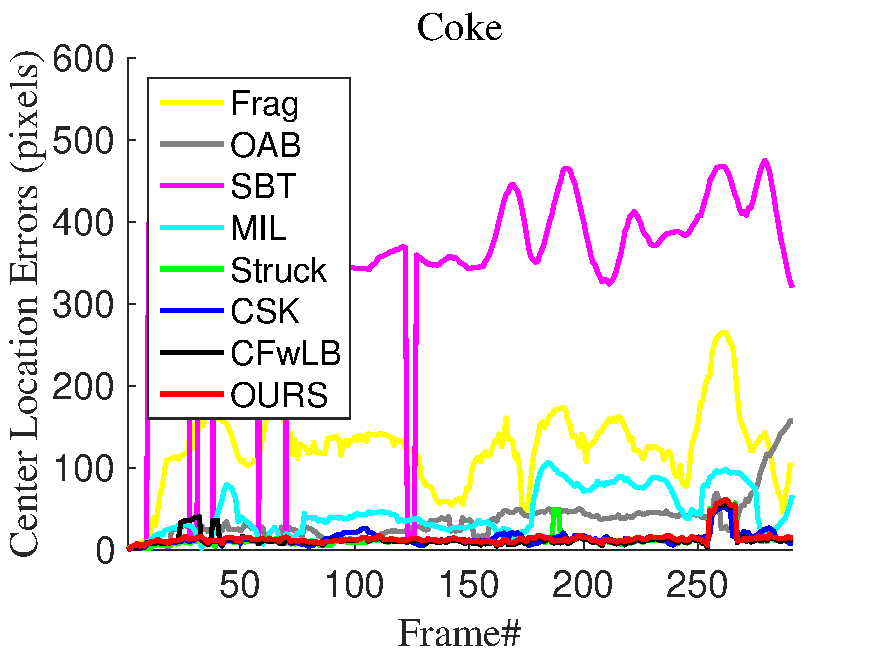
\includegraphics[width=0.3\linewidth]{CFwLB_Coke_prcision.pdf}
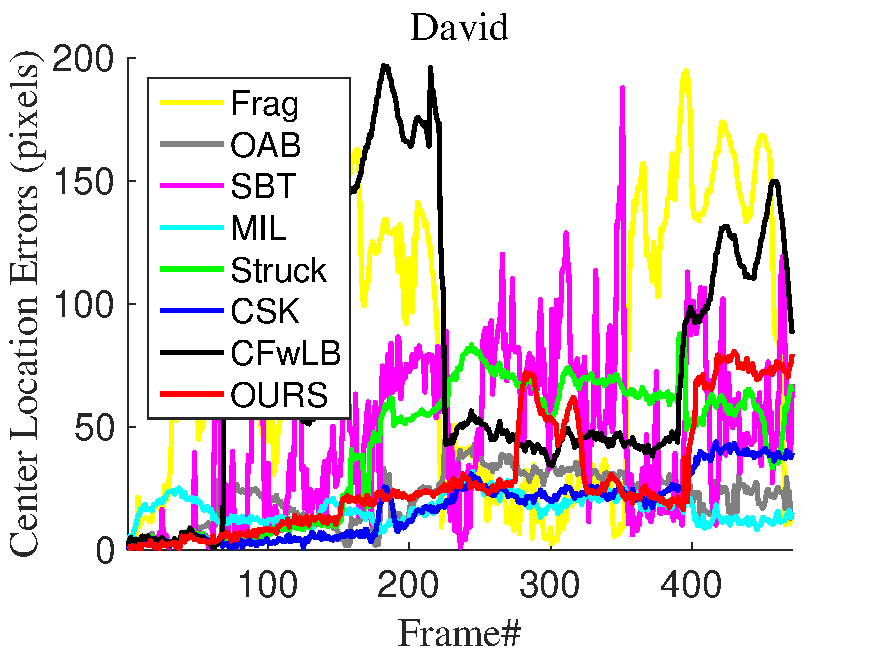
\includegraphics[width=0.3\linewidth]{CFwLB_David_prcision.pdf}
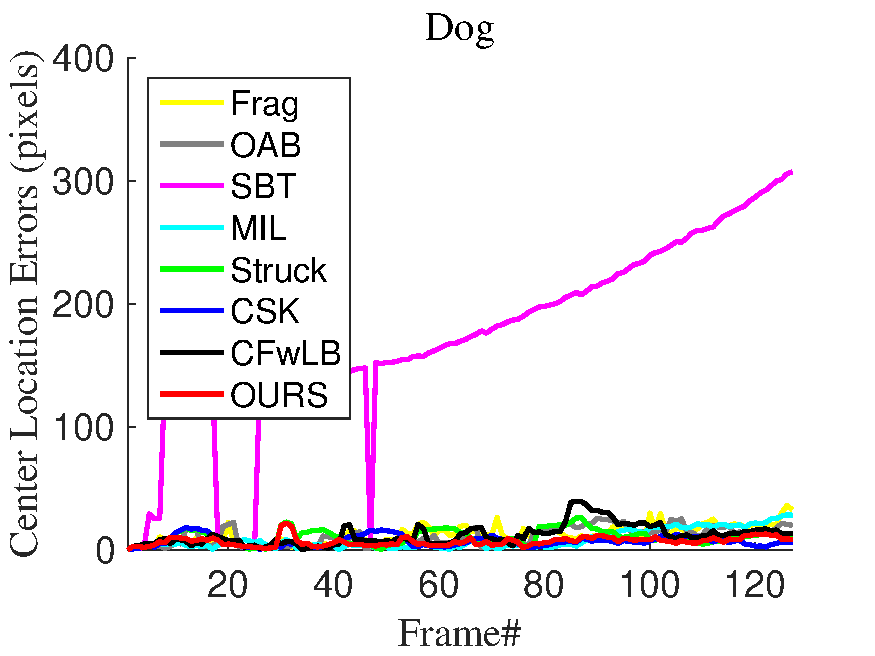
\includegraphics[width=0.3\linewidth]{CFwLB_Dog_prcision.pdf}\\
\includegraphics[width=0.3\linewidth]{CFwLB_Doll_prcision.pdf}
\includegraphics[width=0.3\linewidth]{CFwLB_Gym_prcision.pdf}
\includegraphics[width=0.3\linewidth]{CFwLB_KiteSurf_prcision.pdf}
\end{figure}
\end{frame}
\begin{frame}{中心位置误差对比}
\begin{figure}[htbp]
\centering
\includegraphics[width =0.3\linewidth]{CFwLB_Surfer_prcision.pdf}
\includegraphics[width =0.3\linewidth]{CFwLB_Sylvester_prcision.pdf}
\includegraphics[width =0.3\linewidth]{CFwLB_Vase_prcision.pdf}
\end{figure}
\end{frame}


  \section{评审问题}

\subsection{三种模型的适用范围}

\begin{frame}{赵五老师:}

    \begin{block}{所提出的三个算法分别是解决跟踪算法中的哪些对应的技术难点?请分析说明三种模型的适用范围}
        ~\\
        基于逻辑回归模型的集成学习跟踪从传统方法角度着眼,解决跟踪问题;\\
        自适应目标响应的长时相关滤波跟踪多模块协作,适用于长时跟踪,能够应对复杂场景;\\
        结构化输出的相关滤波跟踪以原始像素为特征,速度约80fps,适用于实时性要求高的环境。
    \end{block}

\end{frame}




{%\xdbg%末页致谢
\begin{frame}[plain,noframenumbering]
 \finalpage{{\huge 谢谢!}}
%{\huge 谢谢!}
\end{frame}}

\end{document} 
